% Options for packages loaded elsewhere
\PassOptionsToPackage{unicode}{hyperref}
\PassOptionsToPackage{hyphens}{url}
%
\documentclass[
]{article}
\usepackage{amsmath,amssymb}
\usepackage{lmodern}
\usepackage{iftex}
\ifPDFTeX
  \usepackage[T1]{fontenc}
  \usepackage[utf8]{inputenc}
  \usepackage{textcomp} % provide euro and other symbols
\else % if luatex or xetex
  \usepackage{unicode-math}
  \defaultfontfeatures{Scale=MatchLowercase}
  \defaultfontfeatures[\rmfamily]{Ligatures=TeX,Scale=1}
\fi
% Use upquote if available, for straight quotes in verbatim environments
\IfFileExists{upquote.sty}{\usepackage{upquote}}{}
\IfFileExists{microtype.sty}{% use microtype if available
  \usepackage[]{microtype}
  \UseMicrotypeSet[protrusion]{basicmath} % disable protrusion for tt fonts
}{}
\makeatletter
\@ifundefined{KOMAClassName}{% if non-KOMA class
  \IfFileExists{parskip.sty}{%
    \usepackage{parskip}
  }{% else
    \setlength{\parindent}{0pt}
    \setlength{\parskip}{6pt plus 2pt minus 1pt}}
}{% if KOMA class
  \KOMAoptions{parskip=half}}
\makeatother
\usepackage{xcolor}
\usepackage[margin=1in]{geometry}
\usepackage{longtable,booktabs,array}
\usepackage{calc} % for calculating minipage widths
% Correct order of tables after \paragraph or \subparagraph
\usepackage{etoolbox}
\makeatletter
\patchcmd\longtable{\par}{\if@noskipsec\mbox{}\fi\par}{}{}
\makeatother
% Allow footnotes in longtable head/foot
\IfFileExists{footnotehyper.sty}{\usepackage{footnotehyper}}{\usepackage{footnote}}
\makesavenoteenv{longtable}
\usepackage{graphicx}
\makeatletter
\def\maxwidth{\ifdim\Gin@nat@width>\linewidth\linewidth\else\Gin@nat@width\fi}
\def\maxheight{\ifdim\Gin@nat@height>\textheight\textheight\else\Gin@nat@height\fi}
\makeatother
% Scale images if necessary, so that they will not overflow the page
% margins by default, and it is still possible to overwrite the defaults
% using explicit options in \includegraphics[width, height, ...]{}
\setkeys{Gin}{width=\maxwidth,height=\maxheight,keepaspectratio}
% Set default figure placement to htbp
\makeatletter
\def\fps@figure{htbp}
\makeatother
\setlength{\emergencystretch}{3em} % prevent overfull lines
\providecommand{\tightlist}{%
  \setlength{\itemsep}{0pt}\setlength{\parskip}{0pt}}
\setcounter{secnumdepth}{-\maxdimen} % remove section numbering
\usepackage{listings}
\lstset{ basicstyle=\footnotesize\ttfamily, breaklines=true, postbreak=\mbox{\textcolor{black}{$\hookrightarrow$}\space}, }
\ifLuaTeX
  \usepackage{selnolig}  % disable illegal ligatures
\fi
\IfFileExists{bookmark.sty}{\usepackage{bookmark}}{\usepackage{hyperref}}
\IfFileExists{xurl.sty}{\usepackage{xurl}}{} % add URL line breaks if available
\urlstyle{same} % disable monospaced font for URLs
\hypersetup{
  pdftitle={PH1976 Project: Predicting Parkinson's Disease for Patients Using Voice Recording},
  pdfauthor={Erin S. King},
  hidelinks,
  pdfcreator={LaTeX via pandoc}}

\title{PH1976 Project: Predicting Parkinson's Disease for Patients Using Voice Recording}
\author{Erin S. King}
\date{2023-04-09}

\begin{document}
\maketitle

{
\setcounter{tocdepth}{2}
\tableofcontents
}
\hypertarget{introduction}{%
\section{Introduction}\label{introduction}}

The following analysis in this PH1976 project is to demonstrate the tools examined in this course for data categorization, regression, and prediction. The project's aim is to predict Parkinson's disease (PD) using the extracted features from the voice recording of patients. For each individual, three recording samples were collected. The \href{https://doi.org/10.1016/j.asoc.2018.10.022}{data and corresponding analysis} is provided by @Sakar in their seminal research on implementing tunable Q-factor wavelet transforms in conjunction with existing data prediction methods. The methods found in this study serve as a roadmap for this project and inform the methods chosen for categorization and prediction.

\hypertarget{definition}{%
\subsection{Definition}\label{definition}}

Parkinson's disease (PD) is a progressive neurodegenerative disorder. To accurately detect the disease in the
early stage, many telediagnosis and telemonitoring systems have recently been proposed. Since vocal problem is
one of the most important symptoms which can be seen in the earlier stage of PD patients, vocal disorders-
based systems become popular in PD diagnosis and monitoring. In these systems, various speech signal
processing algorithms have been used to extract clinically useful information for PD assessment, and the
calculated features are fed to different learning algorithms to make reliable decisions. PD telemedicine studies
showed that the choice of extracted features and learning algorithms directly influences the accuracy and
reliability of distinguishing PD patients.

\hypertarget{data}{%
\subsection{Data}\label{data}}

In this study, Sakar et. al collected the voice recordings of 252 subjects including PD patients and healthy individuals. They gathered three recording samples from each subject and extracted seven feature subsets from the recording samples. The feature subsets were baseline features, intensity-based features, bandwidth and formant features, vocal fold features, Mel Frequency Cepstral Coefficients (MFCC), wavelet transform based features (WT) and tunable Q-factor wavelet transform based features (TQWT).

\hypertarget{study-design}{%
\subsection{Study Design}\label{study-design}}

Need to fill this out based on our own analysis.

\hypertarget{study-population}{%
\subsection{Study Population}\label{study-population}}

The dataset includes PD patients with age ranging from 33 to 87 (65.1 ± 10.9) and healthy individuals with age
ranging from 41 to 82 (61.1 ± 8.9). Each patient has three voice recording samples, with 7 aforementioned
feature subsets. Each feature subset contains several features.

\hypertarget{methods}{%
\section{Methods}\label{methods}}

\hypertarget{preprocessing-and-standardization}{%
\subsection{Preprocessing and Standardization}\label{preprocessing-and-standardization}}

Instead of using the LOOCV method outlined in the paper, we have decided to break the training dataset into a 90/10 split, where 90\% of the data will be used to train, and 10\% of the data will be used to check accuracy of the model. The best model for each subset will be selected based on these results.

For ease of analysis, the ensemble data set (both training and test) are broken into the following sub feature categories:

\begin{itemize}
\tightlist
\item
  Baseline Features
\item
  Time Frequency Features

  \begin{itemize}
  \tightlist
  \item
    Intensity based
  \item
    Formant and Bandwidth based
  \end{itemize}
\item
  Vocal Fold Features
\item
  Mel Frequency Cepstral Coefficients (MFCC)
\item
  Wavelet Transform-based Features
\item
  Tunable Q-Factor Wavelet Transform-based Features (TQWT)
\end{itemize}

Overall, these seven sub features were used to inform the machine learning model and perform predictions on the test set.

To start, data from all sub features are standardized such that each feature has zero mean and unit variance. This was accomplished using the {[}@tidyverse{]}, {[}@broom{]}, and {[}@mosaic{]} packages in RStudio. The histograms below shows an example transformation of the original training data set to the standardized form from the \textbf{Baseline}, \textbf{Intensity}, and \textbf{Formant} sub features. This allows all data comparisons to be made equivalently. To ensure that training and test data are all benchmarked equivalently, mean and standard deviation is calculated using the training data, and is applied to standardize both the training and test data. This way, no information leakage will occur and the models will be provided standardized data that is unbiased.

The authors considered using PCA analysis to perform data reduction and to minimize multi-colinearity, but this ultimately was decided against for clarity. Due to the inherent complexity that comes along with transforming the data set with PCA, the authors opted to use the standardization method above, and implement a subsequent Random Forest (Boruta) factor selection method following the standardization.

\begin{figure}[h]\centering
\caption{baseline Sub-feature: Pre-standardization}
\begin{figure}
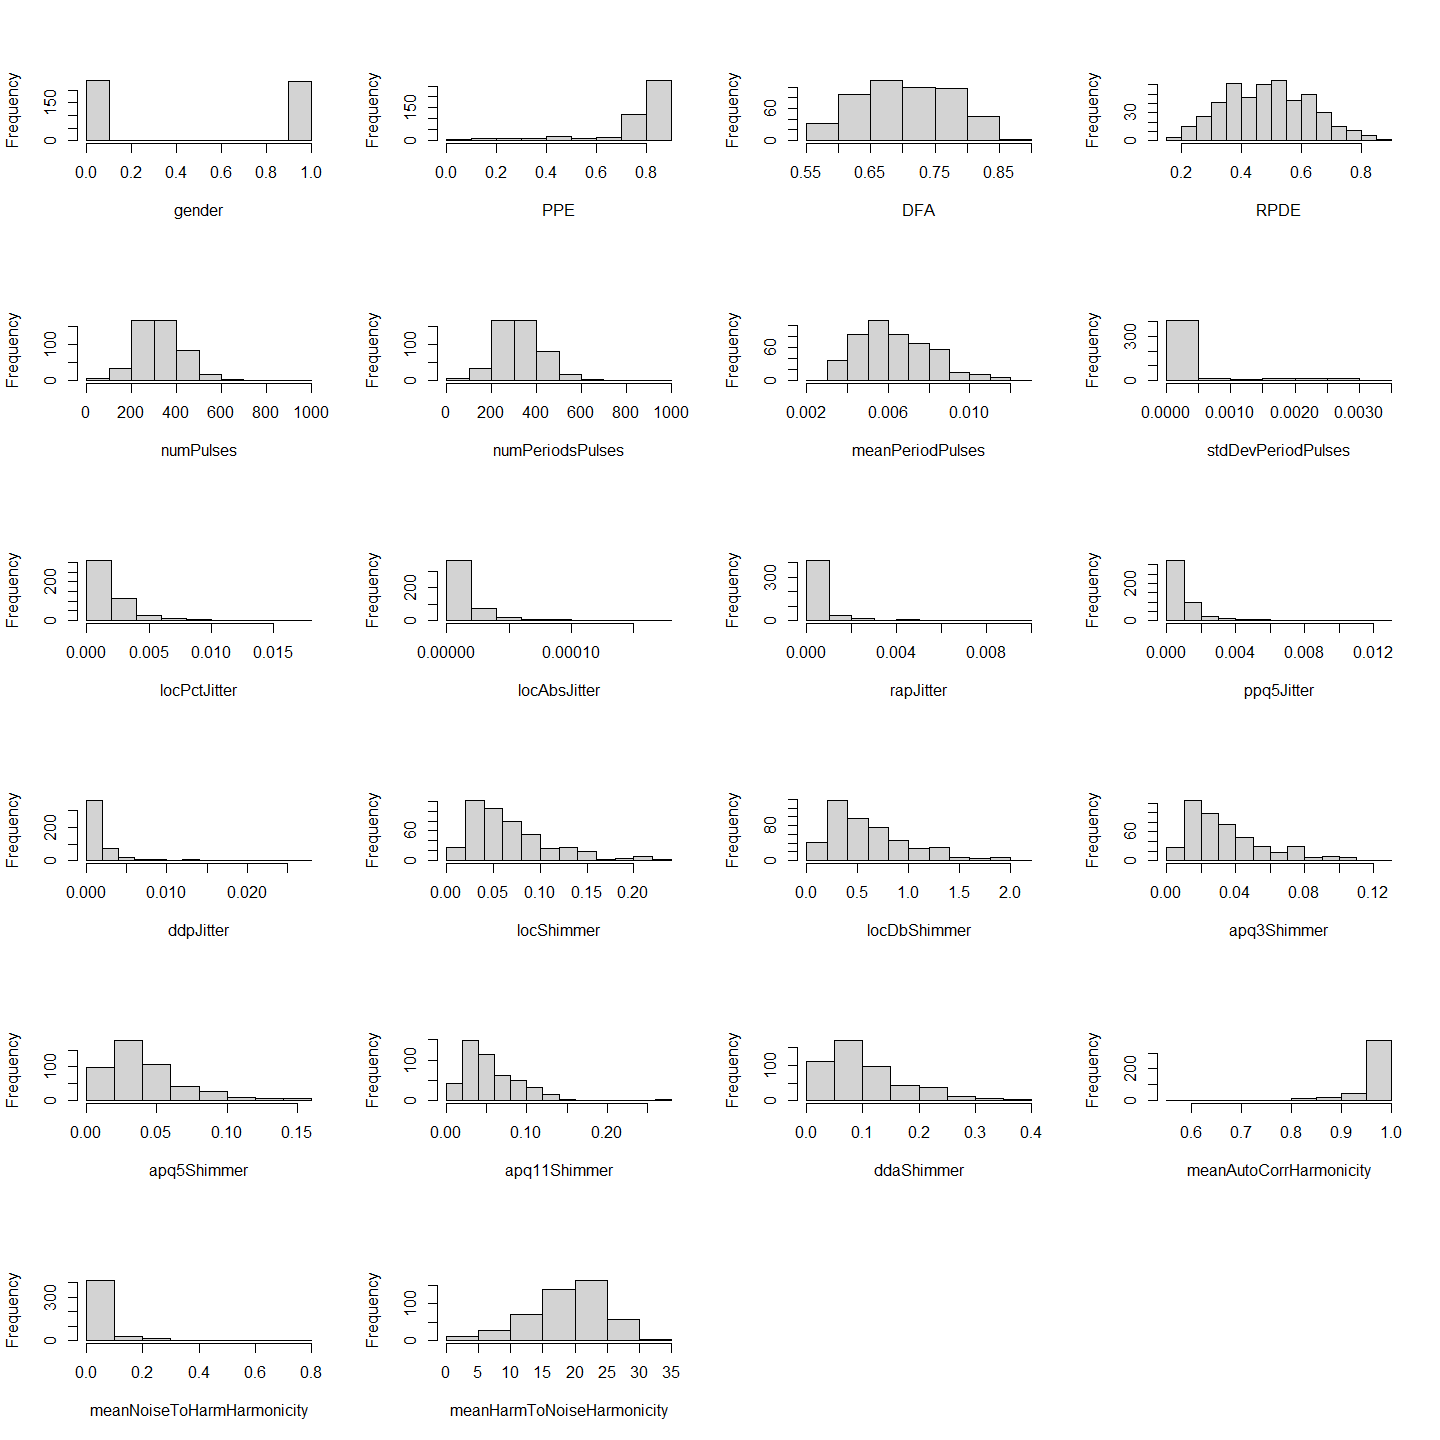
\includegraphics[width=1\linewidth,height=1\textheight]{figure/unnamed-chunk-5-1} \caption{center}\label{fig:unnamed-chunk-5-1}
\end{figure}
\end{figure}
\begin{figure}[h]\centering
\caption{baseline Sub-feature: Post-standardization}
\begin{figure}
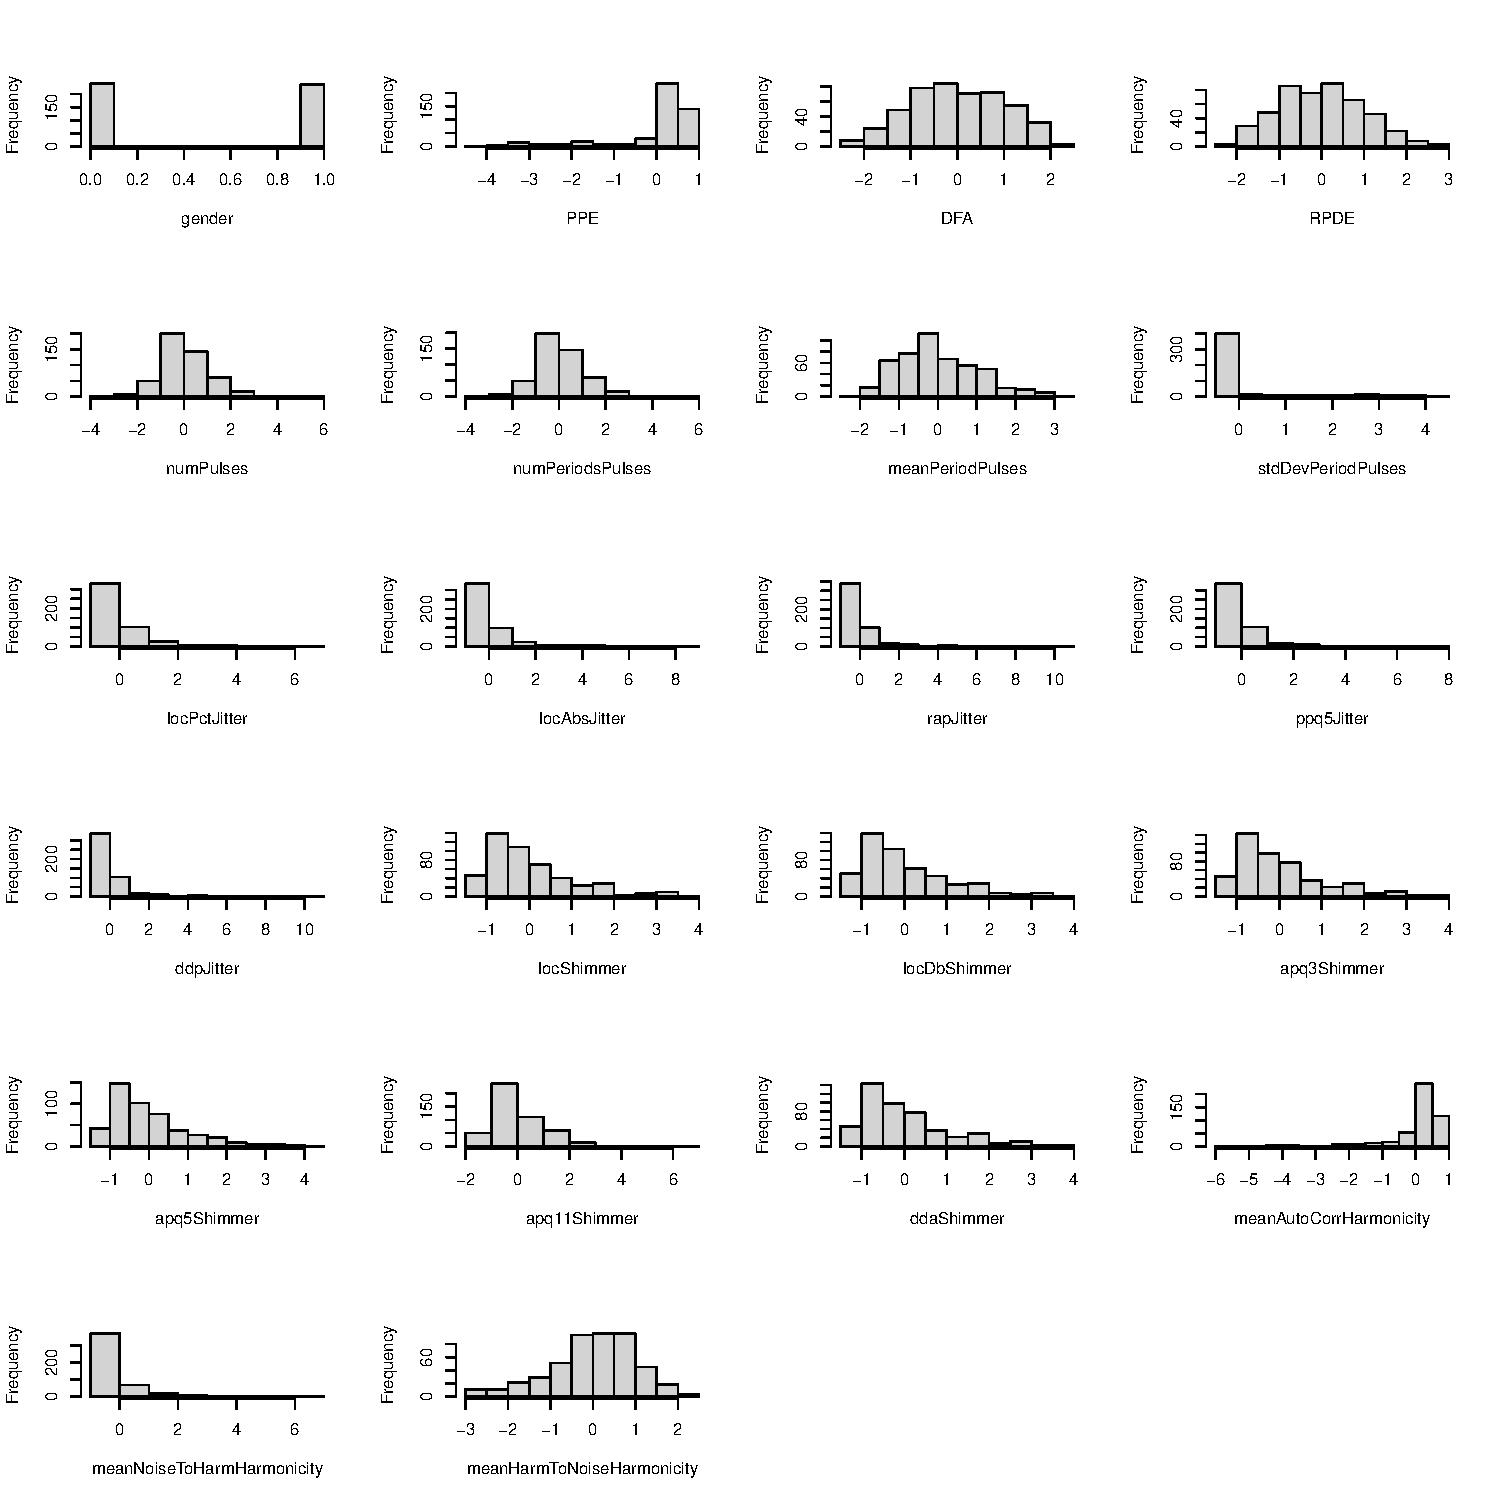
\includegraphics[width=1\linewidth,height=1\textheight]{figure/unnamed-chunk-5-2} \caption{center}\label{fig:unnamed-chunk-5-2}
\end{figure}
\end{figure}
\begin{figure}[h]\centering
\caption{intensity Sub-feature: Pre-standardization}
\begin{figure}
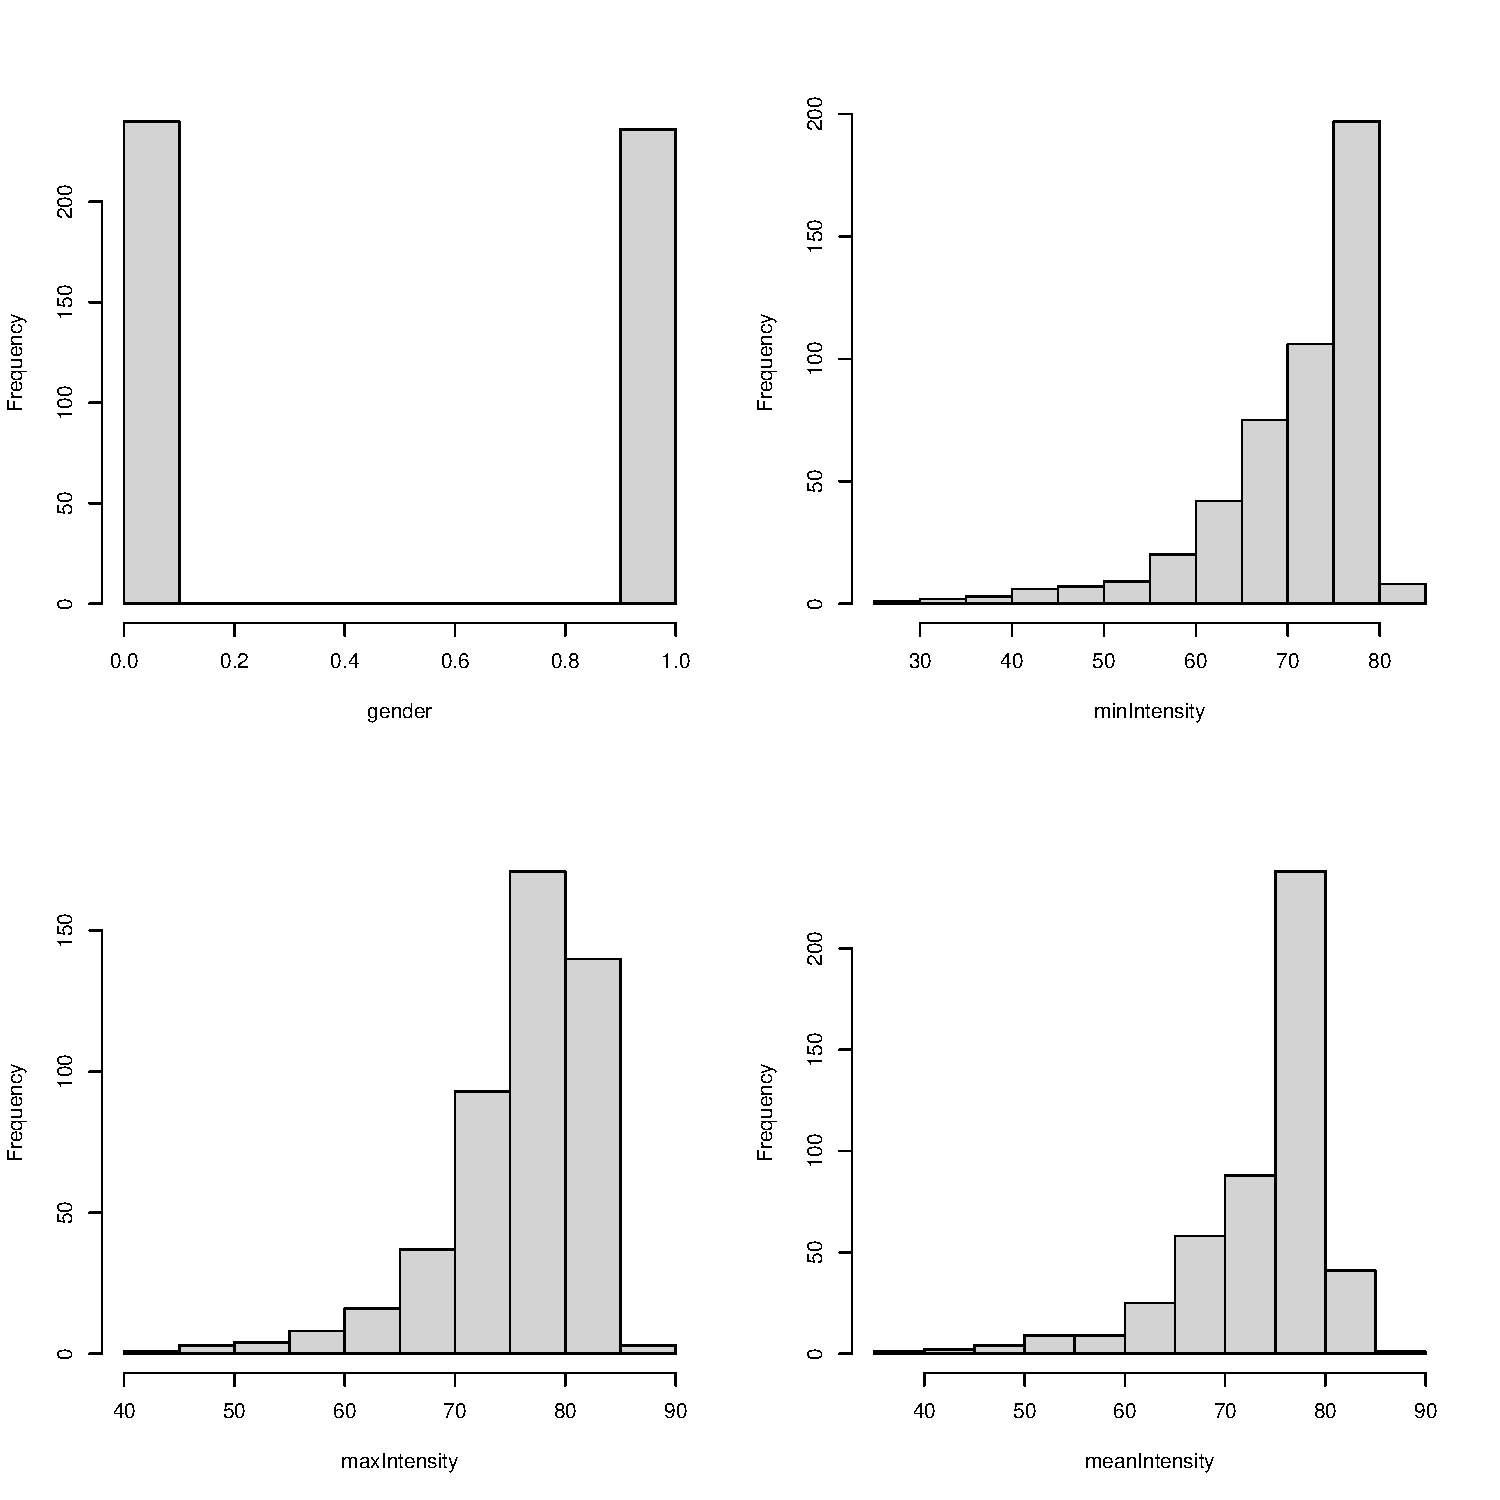
\includegraphics[width=1\linewidth,height=1\textheight]{figure/unnamed-chunk-5-3} \caption{center}\label{fig:unnamed-chunk-5-3}
\end{figure}
\end{figure}
\begin{figure}[h]\centering
\caption{intensity Sub-feature: Post-standardization}
\begin{figure}
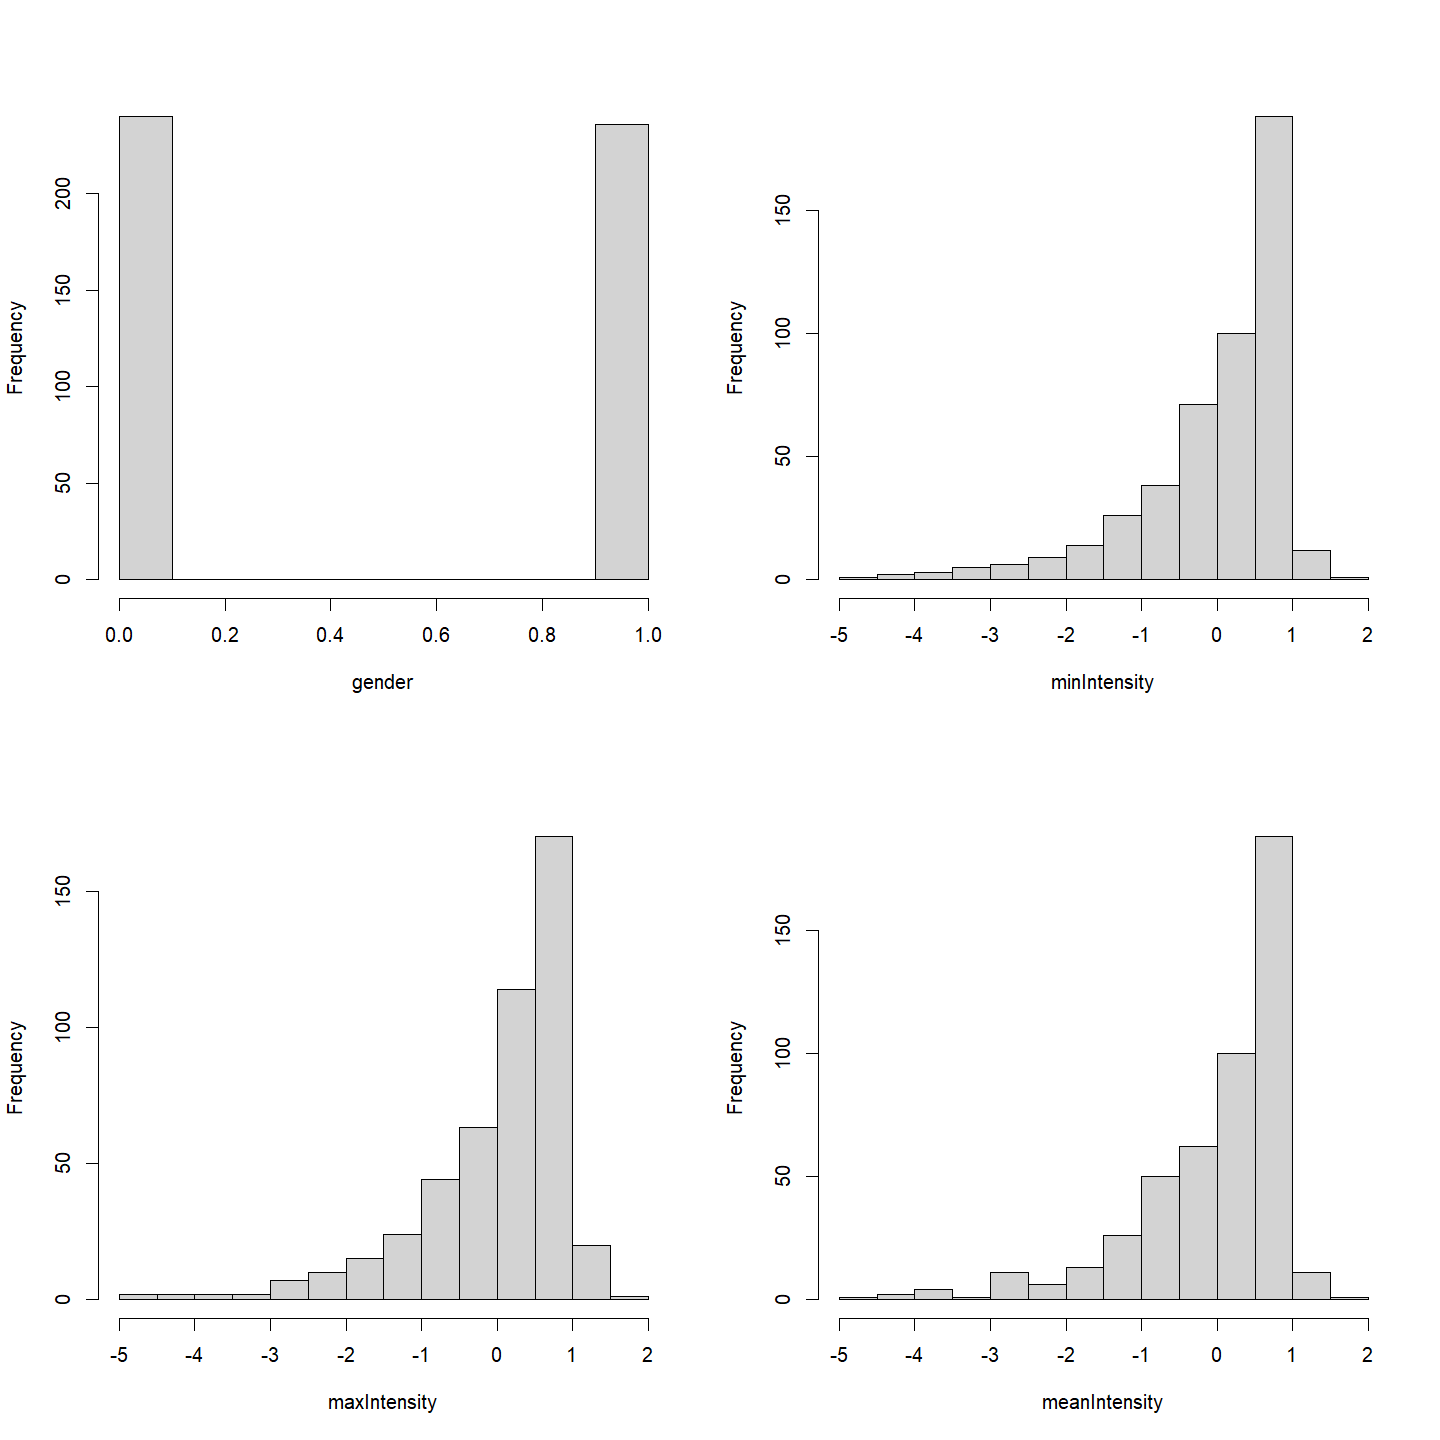
\includegraphics[width=1\linewidth,height=1\textheight]{figure/unnamed-chunk-5-4} \caption{center}\label{fig:unnamed-chunk-5-4}
\end{figure}
\end{figure}
\begin{figure}[h]\centering
\caption{formant Sub-feature: Pre-standardization}
\begin{figure}
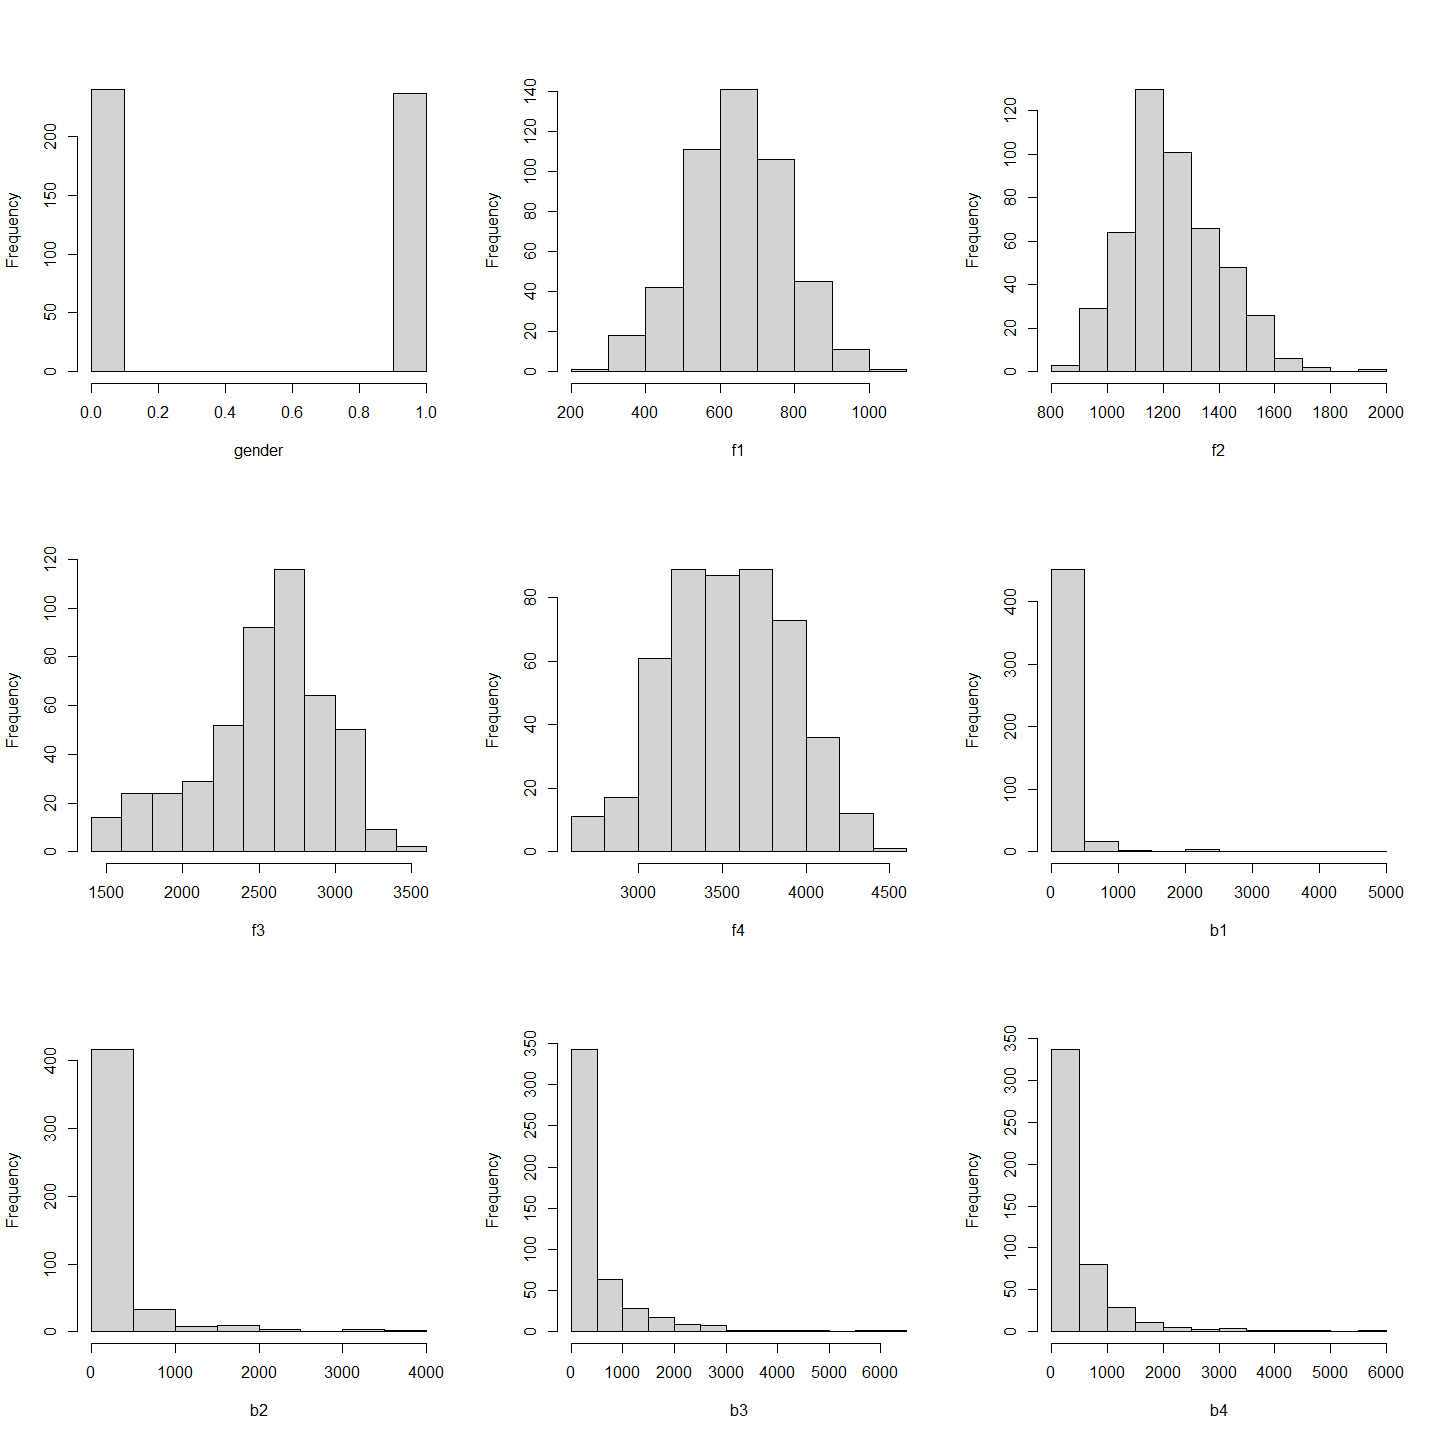
\includegraphics[width=1\linewidth,height=1\textheight]{figure/unnamed-chunk-5-5} \caption{center}\label{fig:unnamed-chunk-5-5}
\end{figure}
\end{figure}
\begin{figure}[h]\centering
\caption{formant Sub-feature: Post-standardization}
\begin{figure}
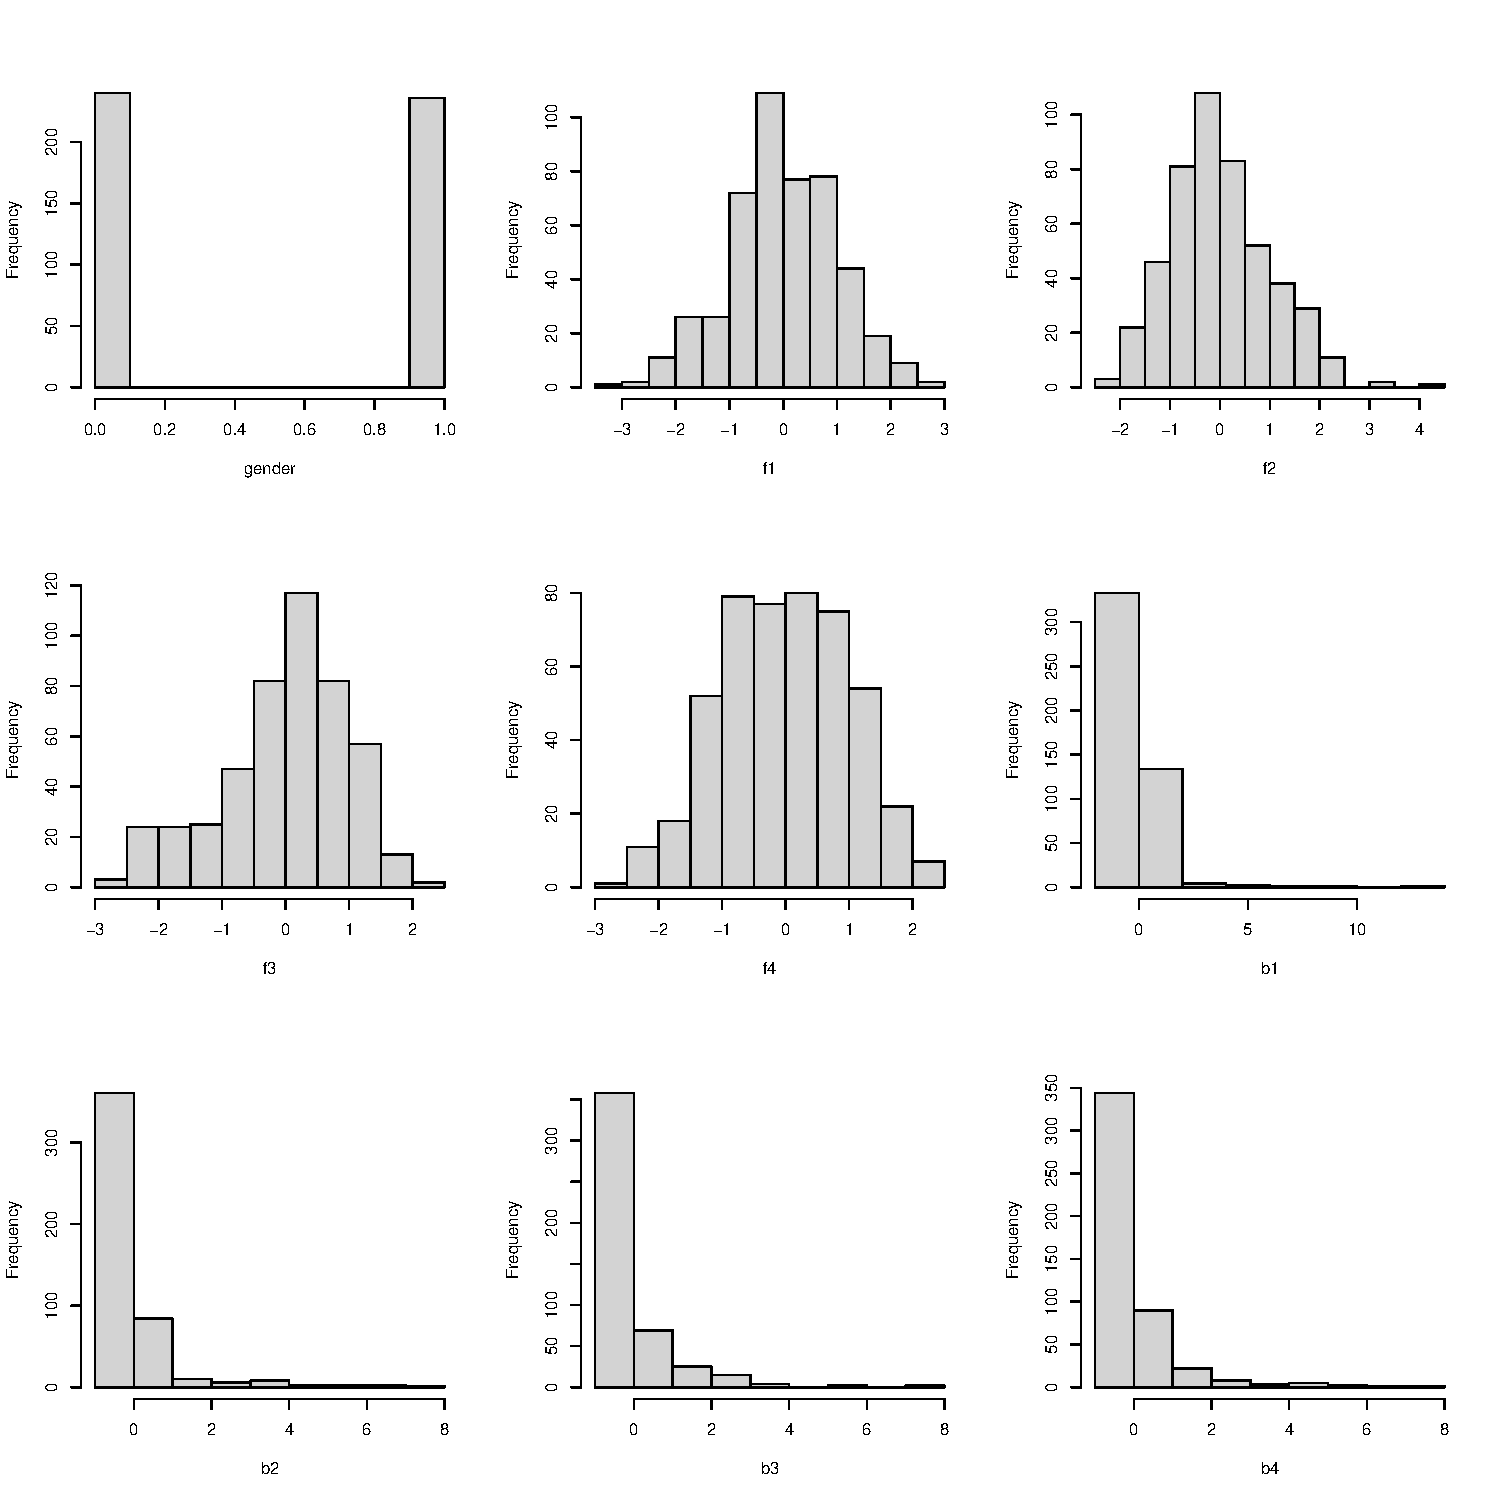
\includegraphics[width=1\linewidth,height=1\textheight]{figure/unnamed-chunk-5-6} \caption{center}\label{fig:unnamed-chunk-5-6}
\end{figure}
\end{figure}

\hypertarget{feature-selection}{%
\subsection{Feature Selection}\label{feature-selection}}

Per the \textbf{Sakar et al} paper, minimum redundancy-maximum relevance based filter feature selection methods are ideal for determining effective features. The advantage of this is two-fold:
1. It reduces the high dimensionality of the data set.
2. It maximizes the joint dependency of the data set.
This strategy is used frequenty in machine learning and regression applications, and as such, will be used in this analysis. The \textbf{Boruta} package in RStudio will be used for this purpose, and utilizes Random Forest to perform a top-down search on the corresponding data frame to determine relevant features.

mRMR analysis yielded the following results. TQWT results are particularly dense, so the plot is not particularly informative, but the overall trend is such that:\\
- Red regions are categorically rejected and excluded from the included features.\\
- Blue regions are tentative, and are handled in a later section of code.\\
- Green regions are found to be imporant and thus selected as included features.

\begin{verbatim}
\begin{figure}[ht!]
\centering
\caption{Boruta plot for baseline features}
\label{fig:boruta_plot_for_baseline_features}
\end{verbatim}

\begin{figure}
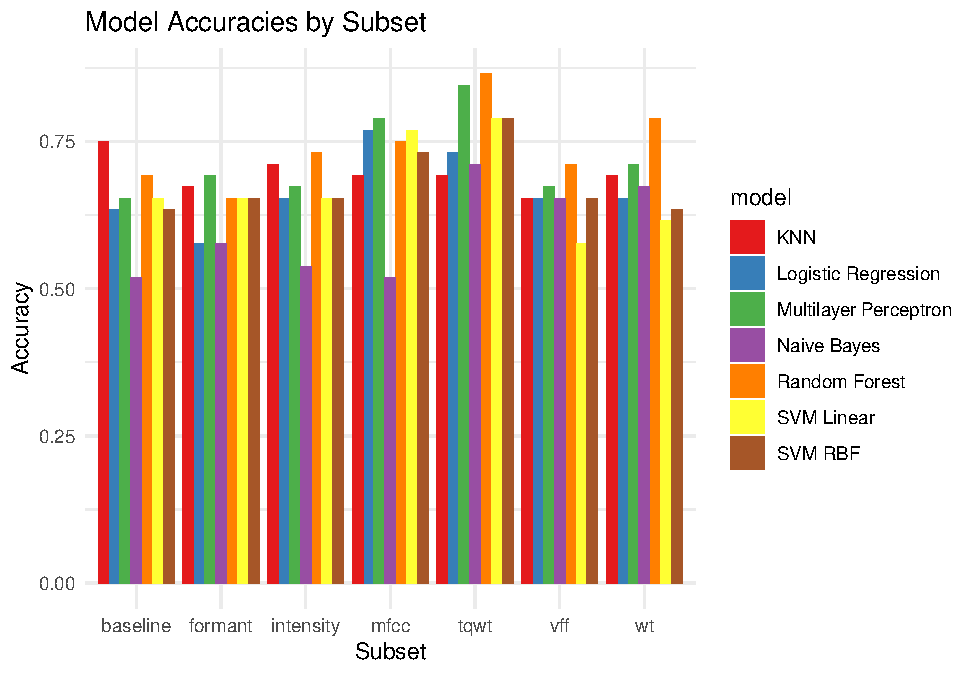
\includegraphics[width=1\linewidth,height=1\textheight]{figure/unnamed-chunk-7-1} \caption{center}\label{fig:unnamed-chunk-7-1}
\end{figure}

\begin{verbatim}
\end{figure}
\begin{figure}[ht!]
\centering
\caption{Boruta plot for intensity features}
\label{fig:boruta_plot_for_intensity_features}
\end{verbatim}

\begin{figure}
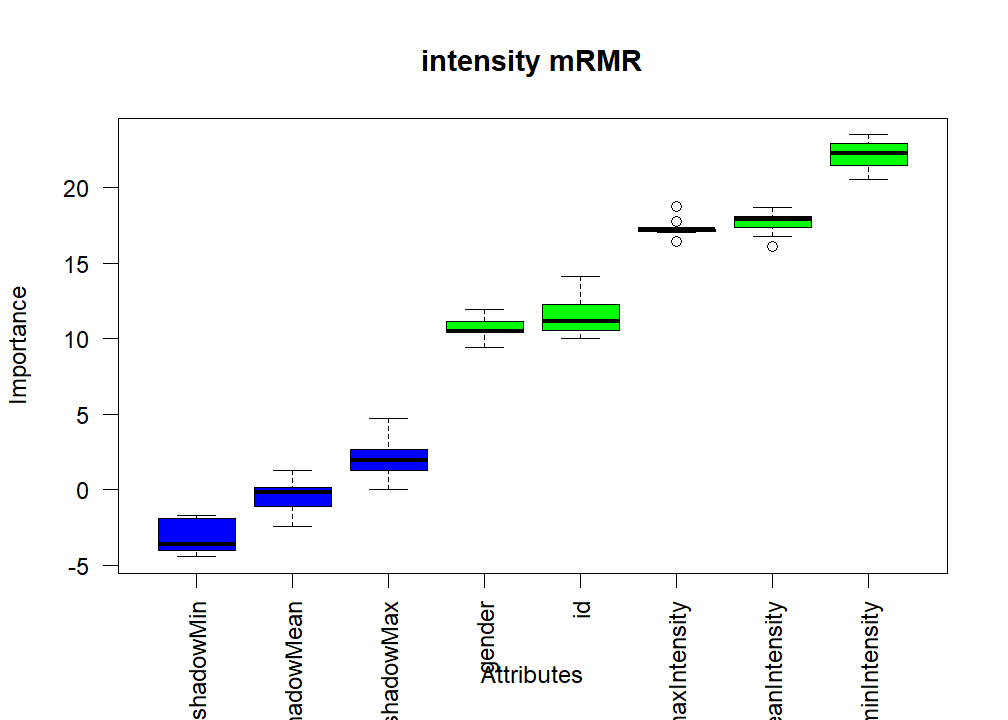
\includegraphics[width=1\linewidth,height=1\textheight]{figure/unnamed-chunk-7-2} \caption{center}\label{fig:unnamed-chunk-7-2}
\end{figure}

\begin{verbatim}
\end{figure}
\begin{figure}[ht!]
\centering
\caption{Boruta plot for formant features}
\label{fig:boruta_plot_for_formant_features}
\end{verbatim}

\begin{figure}
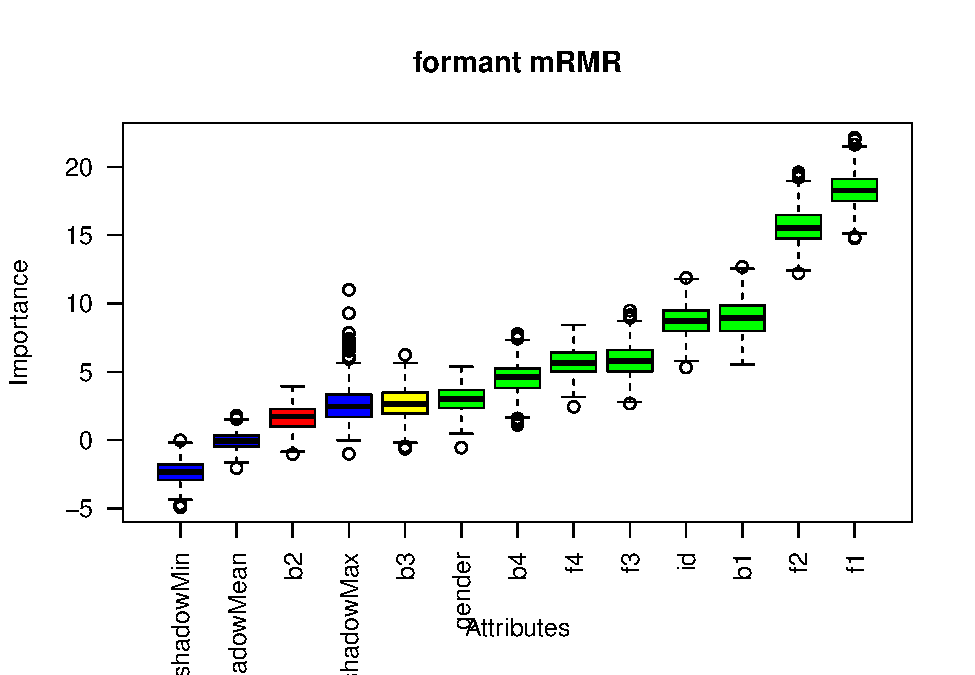
\includegraphics[width=1\linewidth,height=1\textheight]{figure/unnamed-chunk-7-3} \caption{center}\label{fig:unnamed-chunk-7-3}
\end{figure}

\begin{verbatim}
\end{figure}
\begin{figure}[ht!]
\centering
\caption{Boruta plot for vff features}
\label{fig:boruta_plot_for_vff_features}
\end{verbatim}

\begin{figure}
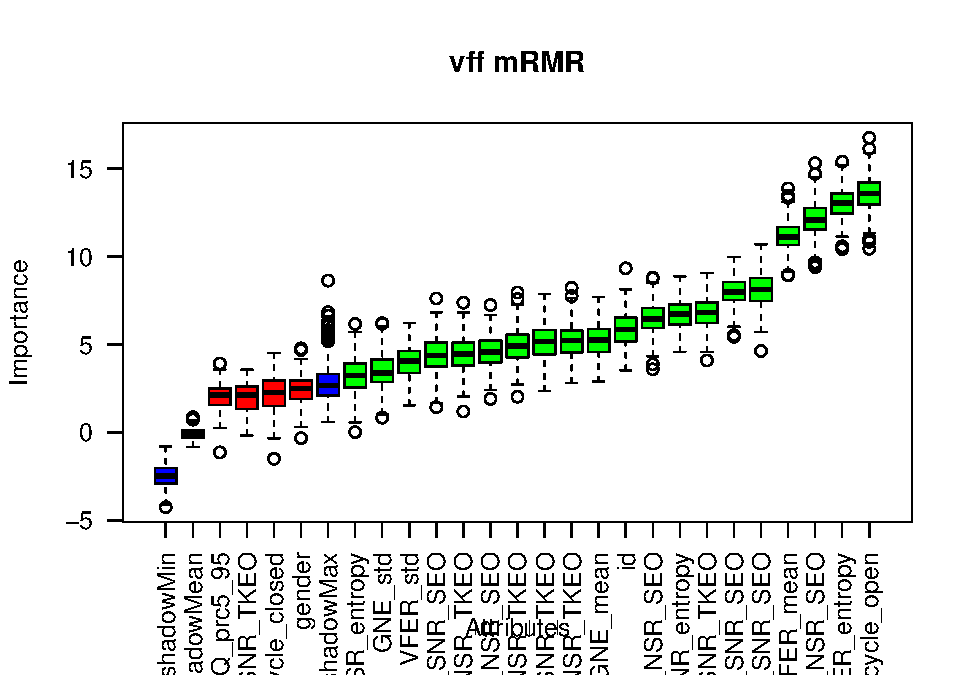
\includegraphics[width=1\linewidth,height=1\textheight]{figure/unnamed-chunk-7-4} \caption{center}\label{fig:unnamed-chunk-7-4}
\end{figure}

\begin{verbatim}
\end{figure}
\begin{figure}[ht!]
\centering
\caption{Boruta plot for mfcc features}
\label{fig:boruta_plot_for_mfcc_features}
\end{verbatim}

\begin{figure}
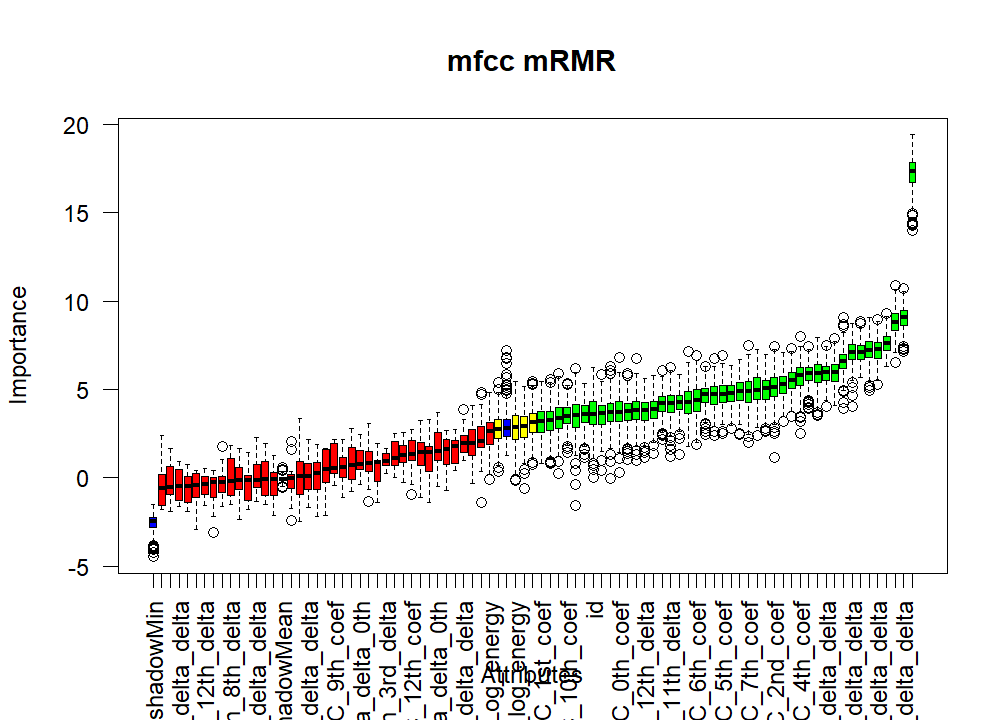
\includegraphics[width=1\linewidth,height=1\textheight]{figure/unnamed-chunk-7-5} \caption{center}\label{fig:unnamed-chunk-7-5}
\end{figure}

\begin{verbatim}
\end{figure}
\begin{figure}[ht!]
\centering
\caption{Boruta plot for wt features}
\label{fig:boruta_plot_for_wt_features}
\end{verbatim}

\begin{figure}
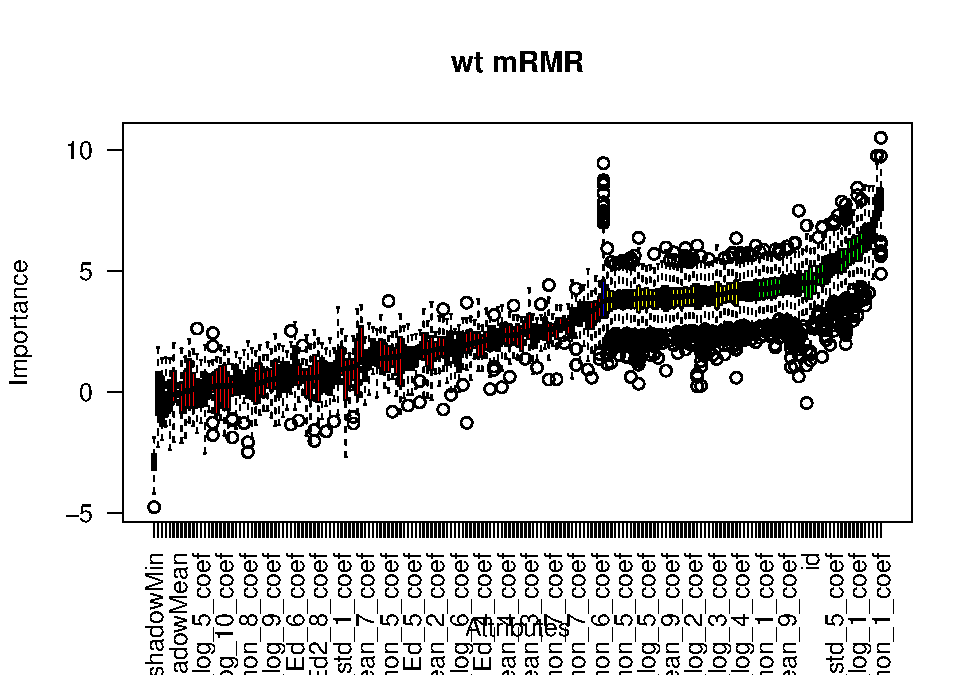
\includegraphics[width=1\linewidth,height=1\textheight]{figure/unnamed-chunk-7-6} \caption{center}\label{fig:unnamed-chunk-7-6}
\end{figure}

\begin{verbatim}
\end{figure}
\begin{figure}[ht!]
\centering
\caption{Boruta plot for tqwt features}
\label{fig:boruta_plot_for_tqwt_features}
\end{verbatim}

\begin{figure}
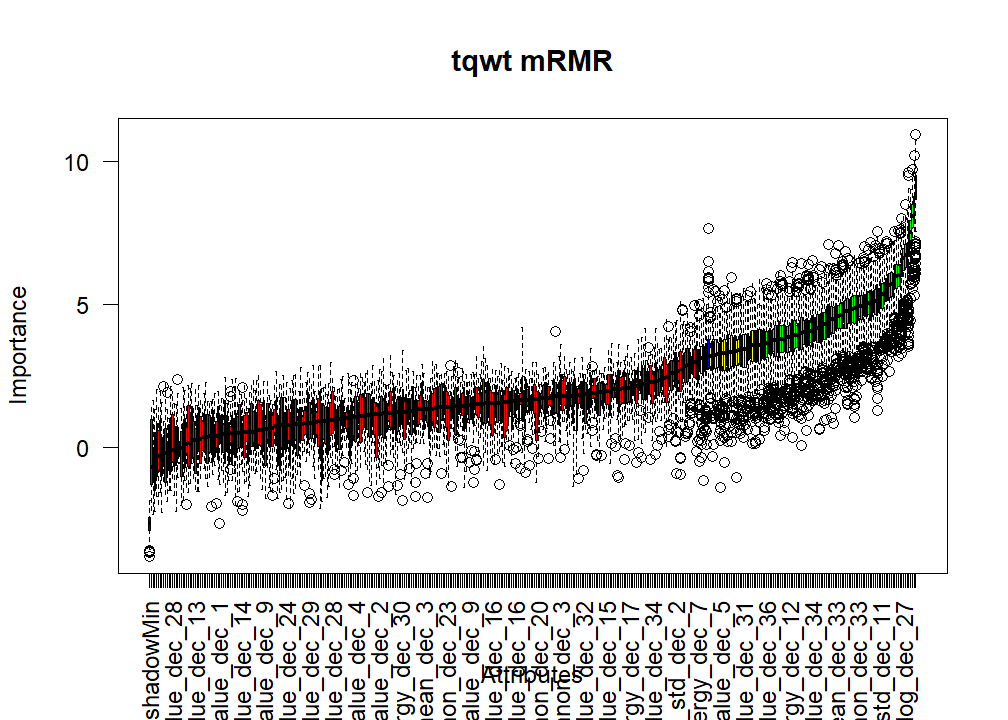
\includegraphics[width=1\linewidth,height=1\textheight]{figure/unnamed-chunk-7-7} \caption{center}\label{fig:unnamed-chunk-7-7}
\end{figure}

\begin{verbatim}
\end{figure}
\end{verbatim}

Following this initial assessment, chosen variables are selected for regression by using \textbf{getNonRejectedFormula()}. This collapses any variables left as \textbf{Tentative} factors into either Accepted or Rejected.

The following factors were found to be important to the model:

\begin{verbatim}
  [1] "class"                          "id"                            
  [3] "DFA"                            "RPDE"                          
  [5] "numPulses"                      "numPeriodsPulses"              
  [7] "meanPeriodPulses"               "stdDevPeriodPulses"            
  [9] "locPctJitter"                   "locAbsJitter"                  
 [11] "rapJitter"                      "ppq5Jitter"                    
 [13] "ddpJitter"                      "locShimmer"                    
 [15] "locDbShimmer"                   "apq3Shimmer"                   
 [17] "apq5Shimmer"                    "apq11Shimmer"                  
 [19] "ddaShimmer"                     "meanAutoCorrHarmonicity"       
 [21] "meanNoiseToHarmHarmonicity"     "meanHarmToNoiseHarmonicity"    
 [23] "gender"                         "minIntensity"                  
 [25] "maxIntensity"                   "meanIntensity"                 
 [27] "f1"                             "f2"                            
 [29] "f3"                             "f4"                            
 [31] "b1"                             "b3"                            
 [33] "b4"                             "GQ_std_cycle_open"             
 [35] "GNE_mean"                       "GNE_std"                       
 [37] "GNE_SNR_TKEO"                   "GNE_SNR_SEO"                   
 [39] "GNE_NSR_TKEO"                   "GNE_NSR_SEO"                   
 [41] "VFER_mean"                      "VFER_std"                      
 [43] "VFER_entropy"                   "VFER_SNR_TKEO"                 
 [45] "VFER_SNR_SEO"                   "VFER_NSR_TKEO"                 
 [47] "VFER_NSR_SEO"                   "IMF_SNR_SEO"                   
 [49] "IMF_SNR_entropy"                "IMF_NSR_SEO"                   
 [51] "IMF_NSR_TKEO"                   "IMF_NSR_entropy"               
 [53] "mean_MFCC_0th_coef"             "mean_MFCC_1st_coef"            
 [55] "mean_MFCC_2nd_coef"             "mean_MFCC_3rd_coef"            
 [57] "mean_MFCC_4th_coef"             "mean_MFCC_5th_coef"            
 [59] "mean_MFCC_6th_coef"             "mean_MFCC_7th_coef"            
 [61] "mean_delta_log_energy"          "mean_2nd_delta"                
 [63] "std_Log_energy"                 "std_MFCC_1st_coef"             
 [65] "std_MFCC_2nd_coef"              "std_MFCC_3rd_coef"             
 [67] "std_MFCC_4th_coef"              "std_MFCC_5th_coef"             
 [69] "std_MFCC_6th_coef"              "std_MFCC_7th_coef"             
 [71] "std_MFCC_8th_coef"              "std_MFCC_10th_coef"            
 [73] "std_MFCC_11th_coef"             "std_delta_log_energy"          
 [75] "std_1st_delta"                  "std_2nd_delta"                 
 [77] "std_3rd_delta"                  "std_4th_delta"                 
 [79] "std_5th_delta"                  "std_6th_delta"                 
 [81] "std_7th_delta"                  "std_8th_delta"                 
 [83] "std_9th_delta"                  "std_10th_delta"                
 [85] "std_11th_delta"                 "std_12th_delta"                
 [87] "std_delta_delta_log_energy"     "std_1st_delta_delta"           
 [89] "std_3rd_delta_delta"            "std_4th_delta_delta"           
 [91] "std_5th_delta_delta"            "std_6th_delta_delta"           
 [93] "std_7th_delta_delta"            "std_8th_delta_delta"           
 [95] "std_9th_delta_delta"            "std_10th_delta_delta"          
 [97] "std_11th_delta_delta"           "std_12th_delta_delta"          
 [99] "Ed_1_coef"                      "Ed_2_coef"                     
[101] "Ed_3_coef"                      "det_entropy_shannon_3_coef"    
[103] "det_entropy_log_1_coef"         "det_entropy_log_2_coef"        
[105] "det_entropy_log_3_coef"         "det_TKEO_mean_1_coef"          
[107] "det_TKEO_std_1_coef"            "det_TKEO_std_3_coef"           
[109] "app_entropy_shannon_1_coef"     "app_entropy_shannon_2_coef"    
[111] "app_entropy_shannon_3_coef"     "app_entropy_shannon_4_coef"    
[113] "app_entropy_shannon_5_coef"     "app_entropy_shannon_9_coef"    
[115] "app_entropy_log_1_coef"         "app_entropy_log_2_coef"        
[117] "app_entropy_log_3_coef"         "app_entropy_log_4_coef"        
[119] "app_entropy_log_5_coef"         "app_entropy_log_6_coef"        
[121] "app_entropy_log_9_coef"         "app_entropy_log_10_coef"       
[123] "app_det_TKEO_mean_4_coef"       "app_det_TKEO_mean_5_coef"      
[125] "app_det_TKEO_mean_8_coef"       "app_det_TKEO_mean_9_coef"      
[127] "app_det_TKEO_mean_10_coef"      "app_TKEO_std_5_coef"           
[129] "app_TKEO_std_6_coef"            "app_TKEO_std_10_coef"          
[131] "Ed2_1_coef"                     "Ed2_2_coef"                    
[133] "Ed2_3_coef"                     "det_LT_entropy_shannon_1_coef" 
[135] "det_LT_entropy_shannon_3_coef"  "det_LT_entropy_log_1_coef"     
[137] "det_LT_entropy_log_3_coef"      "det_LT_TKEO_mean_1_coef"       
[139] "det_LT_TKEO_mean_3_coef"        "det_LT_TKEO_std_1_coef"        
[141] "det_LT_TKEO_std_2_coef"         "det_LT_TKEO_std_3_coef"        
[143] "app_LT_entropy_shannon_1_coef"  "app_LT_entropy_shannon_2_coef" 
[145] "app_LT_entropy_shannon_3_coef"  "app_LT_entropy_shannon_4_coef" 
[147] "app_LT_entropy_shannon_5_coef"  "app_LT_entropy_shannon_6_coef" 
[149] "app_LT_entropy_shannon_8_coef"  "app_LT_entropy_shannon_10_coef"
[151] "app_LT_entropy_log_1_coef"      "app_LT_entropy_log_2_coef"     
[153] "app_LT_entropy_log_3_coef"      "app_LT_entropy_log_4_coef"     
[155] "app_LT_entropy_log_5_coef"      "app_LT_entropy_log_6_coef"     
[157] "app_LT_entropy_log_8_coef"      "app_LT_entropy_log_9_coef"     
[159] "app_LT_entropy_log_10_coef"     "app_LT_TKEO_mean_8_coef"       
[161] "app_LT_TKEO_mean_9_coef"        "app_LT_TKEO_mean_10_coef"      
[163] "app_LT_TKEO_std_5_coef"         "app_LT_TKEO_std_6_coef"        
[165] "app_LT_TKEO_std_7_coef"         "app_LT_TKEO_std_8_coef"        
[167] "app_LT_TKEO_std_9_coef"         "app_LT_TKEO_std_10_coef"       
[169] "tqwt_energy_dec_1"              "tqwt_energy_dec_2"             
[171] "tqwt_energy_dec_6"              "tqwt_energy_dec_11"            
[173] "tqwt_energy_dec_12"             "tqwt_energy_dec_18"            
[175] "tqwt_energy_dec_24"             "tqwt_energy_dec_25"            
[177] "tqwt_energy_dec_26"             "tqwt_energy_dec_27"            
[179] "tqwt_energy_dec_28"             "tqwt_energy_dec_33"            
[181] "tqwt_energy_dec_34"             "tqwt_energy_dec_35"            
[183] "tqwt_entropy_shannon_dec_1"     "tqwt_entropy_shannon_dec_6"    
[185] "tqwt_entropy_shannon_dec_11"    "tqwt_entropy_shannon_dec_12"   
[187] "tqwt_entropy_shannon_dec_13"    "tqwt_entropy_shannon_dec_14"   
[189] "tqwt_entropy_shannon_dec_15"    "tqwt_entropy_shannon_dec_32"   
[191] "tqwt_entropy_shannon_dec_33"    "tqwt_entropy_shannon_dec_34"   
[193] "tqwt_entropy_shannon_dec_35"    "tqwt_entropy_shannon_dec_36"   
[195] "tqwt_entropy_log_dec_1"         "tqwt_entropy_log_dec_12"       
[197] "tqwt_entropy_log_dec_13"        "tqwt_entropy_log_dec_16"       
[199] "tqwt_entropy_log_dec_18"        "tqwt_entropy_log_dec_19"       
[201] "tqwt_entropy_log_dec_25"        "tqwt_entropy_log_dec_26"       
[203] "tqwt_entropy_log_dec_27"        "tqwt_entropy_log_dec_28"       
[205] "tqwt_entropy_log_dec_32"        "tqwt_entropy_log_dec_33"       
[207] "tqwt_entropy_log_dec_34"        "tqwt_entropy_log_dec_35"       
[209] "tqwt_TKEO_mean_dec_2"           "tqwt_TKEO_mean_dec_6"          
[211] "tqwt_TKEO_mean_dec_11"          "tqwt_TKEO_mean_dec_12"         
[213] "tqwt_TKEO_mean_dec_13"          "tqwt_TKEO_mean_dec_18"         
[215] "tqwt_TKEO_mean_dec_19"          "tqwt_TKEO_mean_dec_25"         
[217] "tqwt_TKEO_mean_dec_26"          "tqwt_TKEO_mean_dec_27"         
[219] "tqwt_TKEO_mean_dec_32"          "tqwt_TKEO_mean_dec_33"         
[221] "tqwt_TKEO_mean_dec_34"          "tqwt_TKEO_mean_dec_35"         
[223] "tqwt_TKEO_std_dec_6"            "tqwt_TKEO_std_dec_8"           
[225] "tqwt_TKEO_std_dec_11"           "tqwt_TKEO_std_dec_12"          
[227] "tqwt_TKEO_std_dec_13"           "tqwt_TKEO_std_dec_14"          
[229] "tqwt_TKEO_std_dec_17"           "tqwt_TKEO_std_dec_19"          
[231] "tqwt_TKEO_std_dec_25"           "tqwt_TKEO_std_dec_26"          
[233] "tqwt_TKEO_std_dec_34"           "tqwt_medianValue_dec_31"       
[235] "tqwt_medianValue_dec_34"        "tqwt_meanValue_dec_34"         
[237] "tqwt_meanValue_dec_36"          "tqwt_stdValue_dec_1"           
[239] "tqwt_stdValue_dec_2"            "tqwt_stdValue_dec_5"           
[241] "tqwt_stdValue_dec_6"            "tqwt_stdValue_dec_7"           
[243] "tqwt_stdValue_dec_11"           "tqwt_stdValue_dec_12"          
[245] "tqwt_stdValue_dec_13"           "tqwt_stdValue_dec_18"          
[247] "tqwt_stdValue_dec_19"           "tqwt_stdValue_dec_25"          
[249] "tqwt_stdValue_dec_26"           "tqwt_stdValue_dec_27"          
[251] "tqwt_stdValue_dec_32"           "tqwt_stdValue_dec_33"          
[253] "tqwt_stdValue_dec_34"           "tqwt_stdValue_dec_35"          
[255] "tqwt_minValue_dec_7"            "tqwt_minValue_dec_11"          
[257] "tqwt_minValue_dec_12"           "tqwt_minValue_dec_13"          
[259] "tqwt_minValue_dec_14"           "tqwt_minValue_dec_17"          
[261] "tqwt_maxValue_dec_6"            "tqwt_maxValue_dec_11"          
[263] "tqwt_maxValue_dec_12"           "tqwt_maxValue_dec_13"          
[265] "tqwt_maxValue_dec_14"           "tqwt_maxValue_dec_17"          
[267] "tqwt_skewnessValue_dec_24"      "tqwt_skewnessValue_dec_25"     
[269] "tqwt_skewnessValue_dec_26"      "tqwt_skewnessValue_dec_27"     
[271] "tqwt_kurtosisValue_dec_12"      "tqwt_kurtosisValue_dec_16"     
[273] "tqwt_kurtosisValue_dec_17"      "tqwt_kurtosisValue_dec_18"     
[275] "tqwt_kurtosisValue_dec_19"      "tqwt_kurtosisValue_dec_20"     
[277] "tqwt_kurtosisValue_dec_22"      "tqwt_kurtosisValue_dec_25"     
[279] "tqwt_kurtosisValue_dec_26"      "tqwt_kurtosisValue_dec_27"     
[281] "tqwt_kurtosisValue_dec_29"      "tqwt_kurtosisValue_dec_32"     
[283] "tqwt_kurtosisValue_dec_33"      "tqwt_kurtosisValue_dec_34"     
[285] "tqwt_kurtosisValue_dec_35"     
\end{verbatim}

\hypertarget{model-selection}{%
\subsection{Model Selection}\label{model-selection}}

Once the important features had been determined, they can be used to inform the predictive model for each sub-group.
For this analysis, a function was built to test each sub-group against a number of predictive models. Using the 10\% ``test'' data of the training set, accuracy estimates were generated and used to benchmark the model's performance against each other. The models used for analysis were:\\
- Multilayer Perceptron\\
- Logistic Regression\\
- SVM w/ Linear Kernel\\
- SVM w/ Radial Kernel\\
- Naive Bayes\\
- k- Nearest Neighbors

For this analysis it required the use of the \textbf{caret}, \textbf{randomForest}, \textbf{e1071}, \textbf{nnet}, \textbf{kernlab}, and \textbf{naivebayes} libraries.

The following results were found for each of the sub features. A comparative bar chart for each of the sub features is also included.

\begin{verbatim}
Best model for baseline is KNN with an accuracy of 0.75 
Best model for intensity is Random Forest with an accuracy of 0.7307692 
Best model for formant is Multilayer Perceptron with an accuracy of 0.6923077 
Best model for vff is Random Forest with an accuracy of 0.7115385 
Best model for mfcc is Multilayer Perceptron with an accuracy of 0.7884615 
Best model for wt is Random Forest with an accuracy of 0.7884615 
Best model for tqwt is Random Forest with an accuracy of 0.8653846 
\end{verbatim}

\begin{figure}
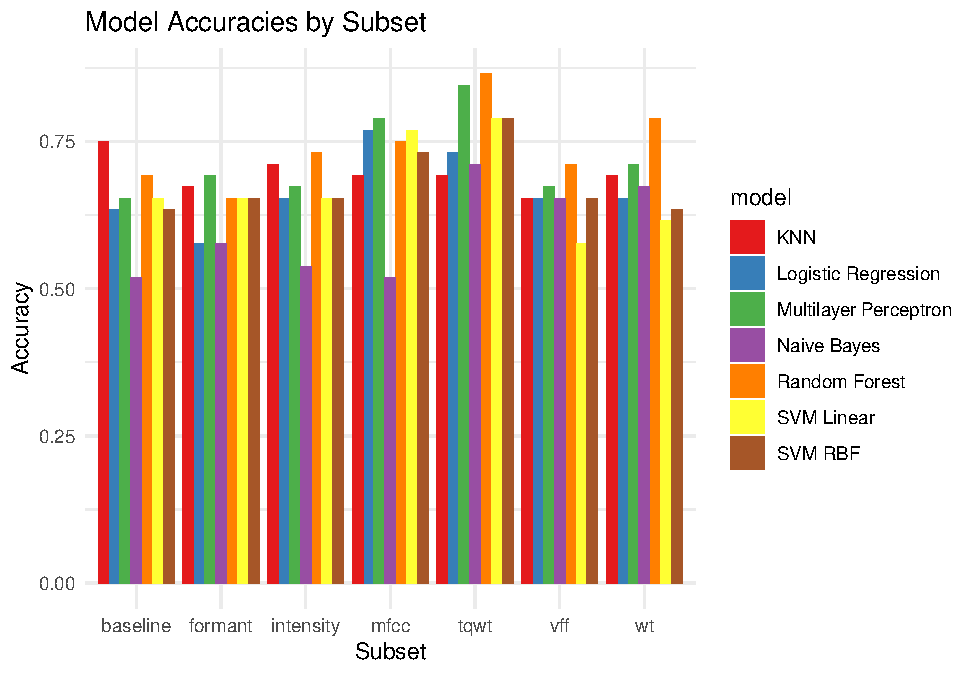
\includegraphics[width=1\linewidth,height=1\textheight]{figure/unnamed-chunk-12-1} \caption{center}\label{fig:unnamed-chunk-12}
\end{figure}

At this point, we have enough data to make an ensemble predictive model, such that the best performing model for each subfeature can be used.

\begin{verbatim}
Ensemble model accuracy: 0.7692308 
\end{verbatim}

\hypertarget{results}{%
\section{Results}\label{results}}

Will update with the model output at a later date.

\end{document}
